\chapter{Logical Mapping}

We have discussed the E-R diagram, which represents the \textbf{conceptual schema}. Once we have the E-R diagram, we can derive a \textbf{relational diagram}.  

\section{Relational Model}
Let us first take a look at the \textbf{relational model}.  

\subsection{Relation}
A \textbf{relation} consists of a \textbf{relation schema} and its \textbf{relation instance}. One can think of a relation as an \emph{entity set}, where the relation instance is the set of records that populate the relation and corresponds to the entities in that set.  

A \textbf{relation schema} describes the column headers for the table. It specifies the relation's name, the name of each field, and, if detailed, the domain of each field. 

More formally, a relation schema \(R\) is a finite set of attribute names:  
\[
R = (A_1, A_2, \dots, A_n)
\]  

For each attribute name \(A_i\), there is a corresponding \textbf{domain} \(D_i\), which is the set of values that \(A_i\) can take. Attribute values are required to be \textbf{atomic} (indivisible). The value \texttt{NULL} is also considered a member of every domain.

A relation \(r\) on the relation schema \(R\) is a subset of \(D = D_1 \times D_2 \times \cdots \times D_n\). Thus, a relation is a set of \(n\)-tuples \((a_1, a_2, \dots, a_n)\) where each \(a_i \in D_i\). The current values (instance) of a relation are specified by a table. An element \(t\) of \(r\) is called a \textbf{tuple} and is represented by a row in the table.

The relational model requires that no two rows be identical. Thus, a relation is defined as a set of unique tuples (rows). This implies that the order in which the rows are listed, as well as the order of the fields, is not important.

\begin{remark}
An unordered collection of elements is called a \emph{set}, while an ordered collection of elements is called a \emph{list}.
\end{remark}

In the relational model, the concept of \textbf{keys} remains fundamental.

In the relational model, relationships are represented using \textbf{foreign keys}. A foreign key is an attribute (or a set of attributes) in one relation that refers to the primary key of another relation.  

Formally, a set of attributes \(FK\) in a relation schema \(R_1\) is a foreign key if these attributes have the same domains as the attributes of the primary key in another relation schema \(R_2\), and for each tuple \(t_1 \in R_1\), the value of \(FK\) either matches the value of the primary key in some tuple \(t_2 \in R_2\), or is \texttt{NULL}.  

\section{Mapping Process}
After introducing the terminology, we now examine how to derive a relational schema from an E-R diagram.

\subsubsection{Step 1: Strong Entities}
For each strong (or regular) entity type \(E\), create a new relation \(R\).  
\begin{itemize}
  \item The attributes of \(R\) include all simple attributes (and simple components of composite attributes) of \(E\).  
  \item The primary key of \(R\) is the key of \(E\).  
\end{itemize}

\subsubsection{Step 2: Weak Entities}
For each weak entity type \(W\) with the identifying (owner) entity type \(E\):  
\begin{itemize}
  \item Create a new relation \(R\).  
  \item The attributes of \(R\) include all simple attributes (and simple components of composite attributes) of \(W\), as well as the primary key attributes of the relation derived from \(E\).  
  \item The key of \(R\) is the combination of the foreign key to \(E\) and the partial key of \(W\).  
\end{itemize}

\subsubsection{Step 3: One-to-One Relationships}
For each one-to-one relationship type \(B\), let \(S\) and \(T\) be the participating entity types. Choose one of them (say \(S\)) — preferably the one with total participation.  
\begin{itemize}
  \item Add the primary key attributes of \(T\) to the relation corresponding to \(S\) as a foreign key.  
  \item Add all simple attributes (and simple components of composite attributes) of \(B\) to \(S\).  
\end{itemize}

\subsubsection{Step 4: One-to-Many Relationships}
For each one-to-many relationship type \(B\), let \(S\) and \(T\) be the participating entity types, where \(S\) is on the “one” side and \(T\) on the “many” side.  
\begin{itemize}
  \item Add to the relation corresponding to \(T\) the primary key attributes of \(S\) as a foreign key.  
  \item Add any simple attributes (or simple components of composite attributes) from the relationship \(B\).  
\end{itemize}

\subsubsection{Step 5: Many-to-Many Relationships}
For each many-to-many relationship type \(B\), let \(S\) and \(T\) be the participating entity types.  
\begin{itemize}
  \item Create a new relation \(R\).  
  \item The attributes of \(R\) include the primary key attributes of \(S\) and \(T\) (as foreign keys), and all simple attributes (and simple components of composite attributes) of \(B\).  
  \item The primary key of \(R\) is the combination of the keys of \(S\) and \(T\).  
\end{itemize}

\subsubsection{Step 6: Multivalued Attributes}
For each multivalued attribute \(A\) of an entity \(E\):  
\begin{itemize}
  \item Create a new relation \(R\).  
  \item If \(A\) is a multivalued simple attribute, the attributes of \(R\) are \(A\) and the primary key of \(E\) (as a foreign key).  
  \item If \(A\) is a multivalued composite attribute, the attributes of \(R\) are all simple components of \(A\) and the primary key of \(E\) (as a foreign key).  
  \item The primary key of \(R\) is the combination of all attributes in \(R\).  
\end{itemize}

\subsubsection{Step 7: N-ary Relationships}
For each \(n\)-ary relationship type (\(n > 2\)):  
\begin{itemize}
  \item Create a new relation \(R\) using the same approach as for many-to-many relationships.  
  \item However, if one of the participating entity types has a participation ratio of 1, its key may serve as the primary key for \(R\).  
\end{itemize}

\begin{figure}[H]
  \centering
  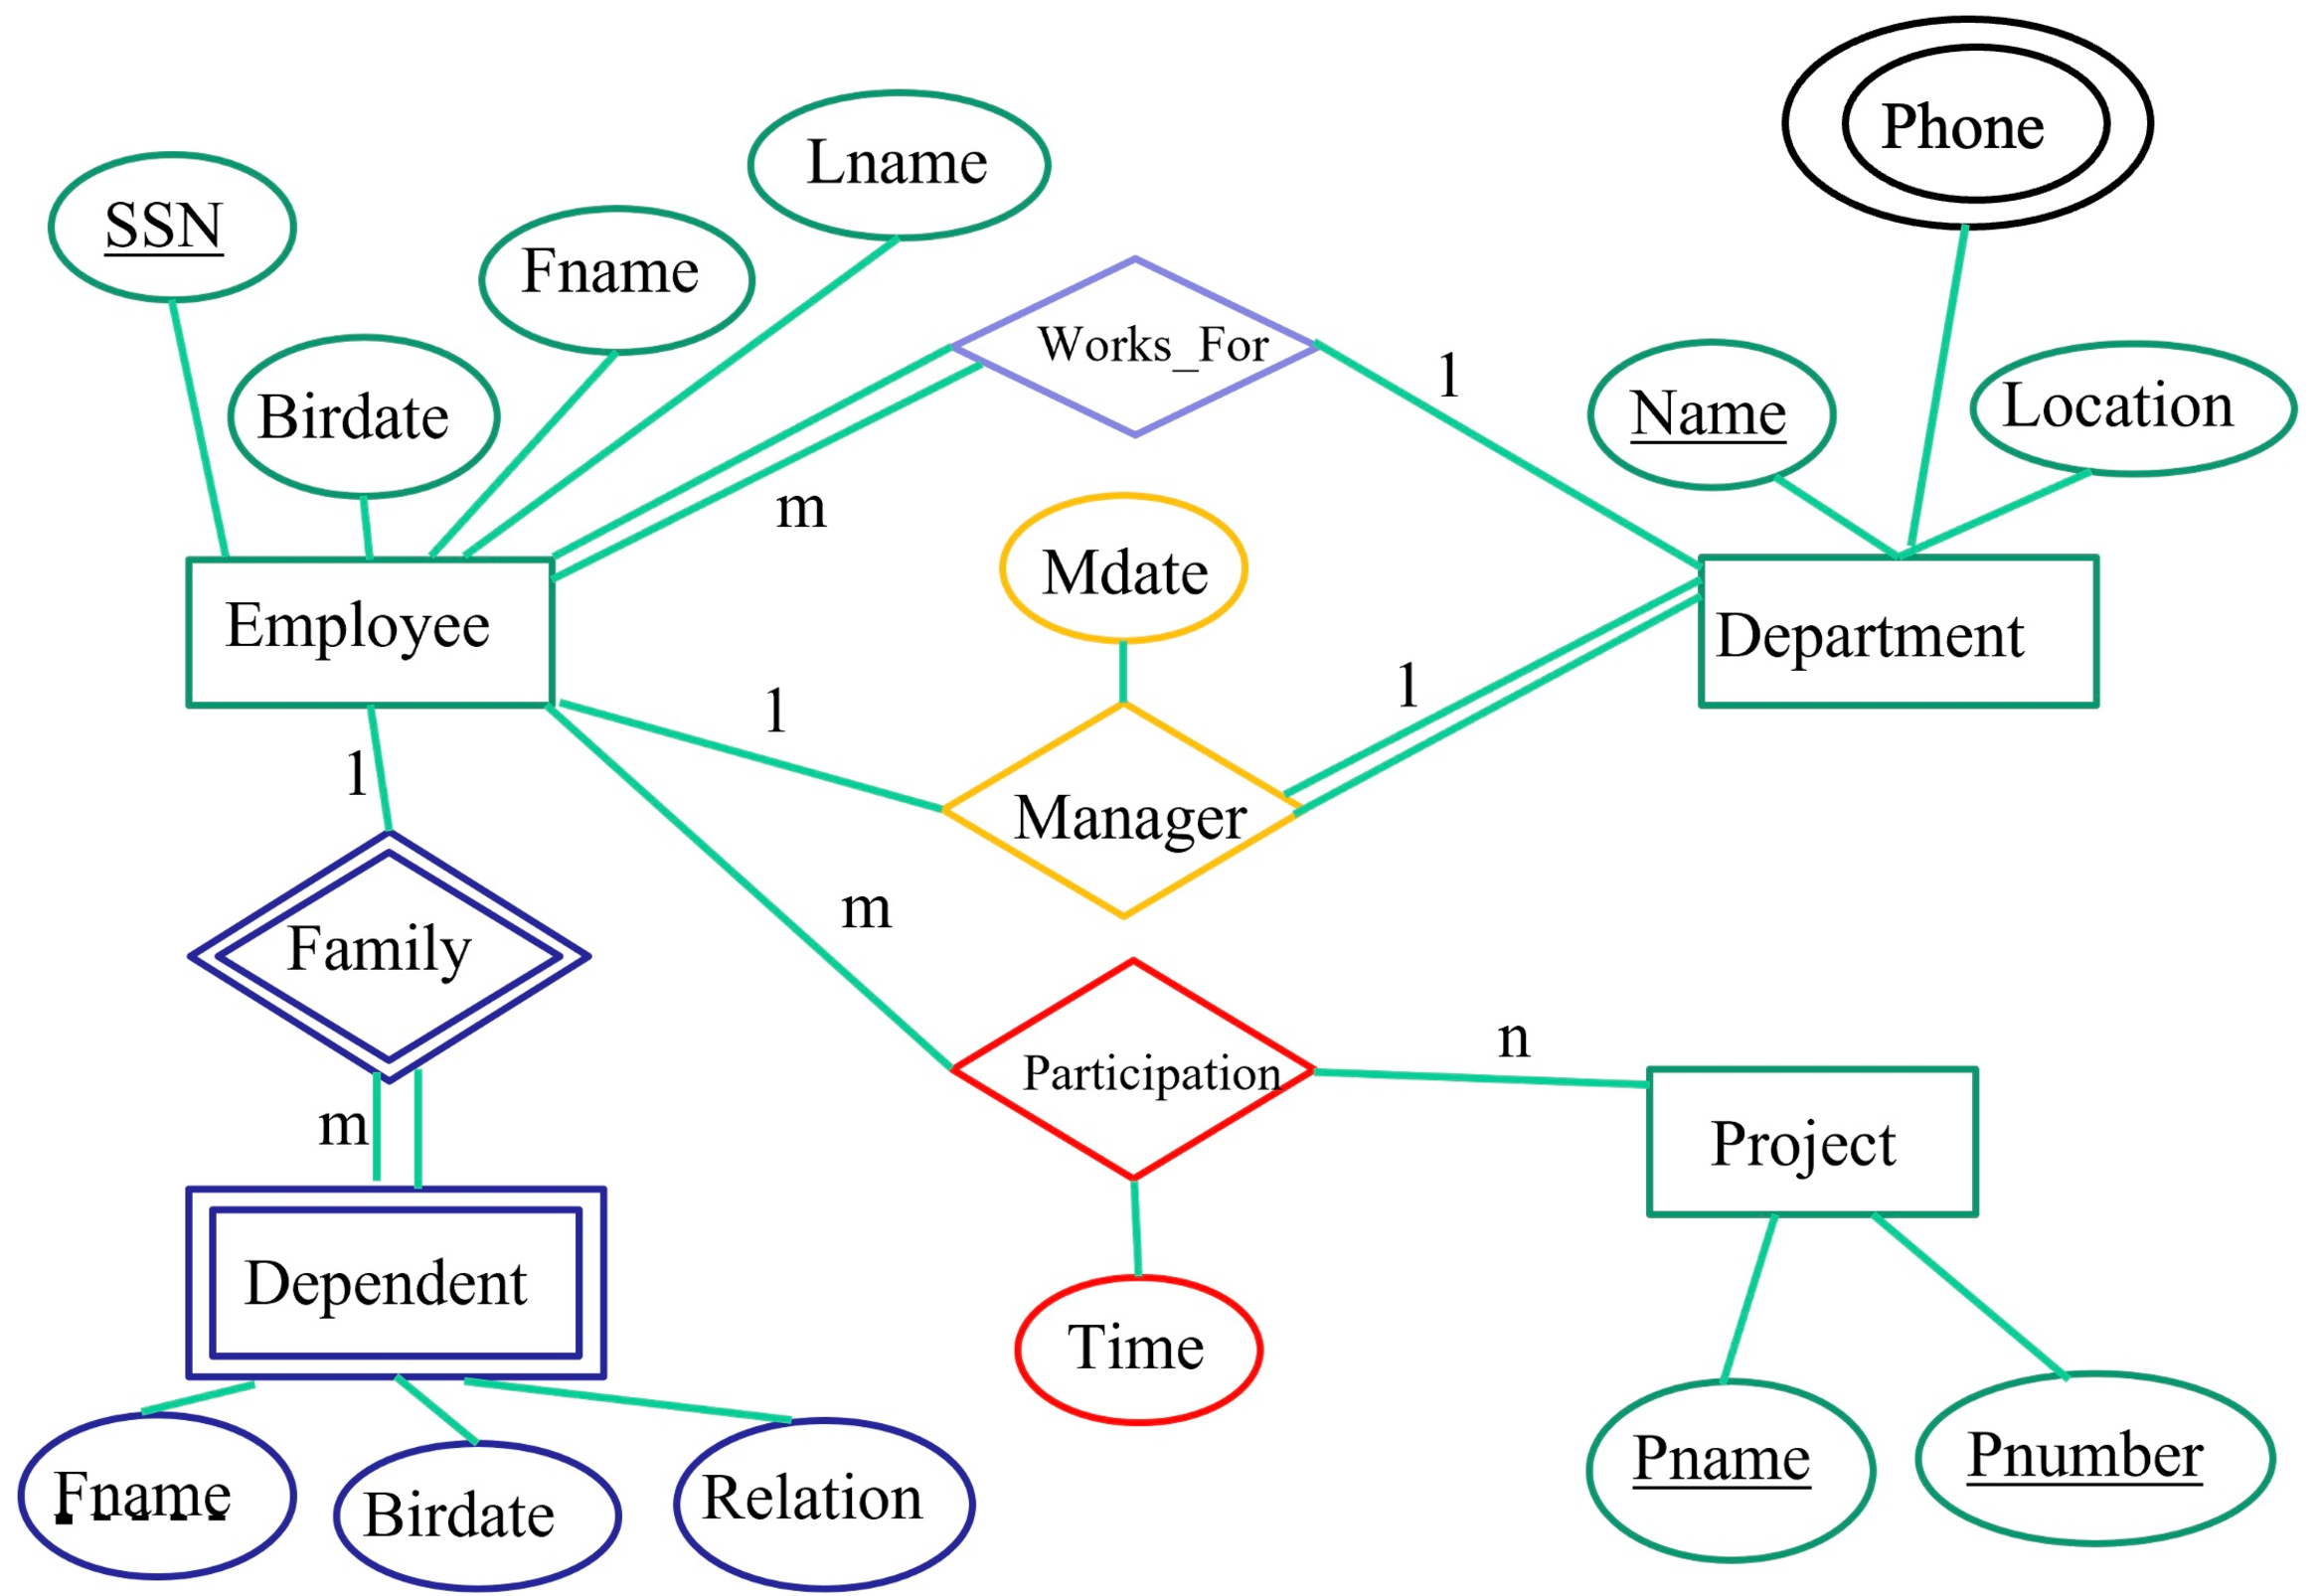
\includegraphics[width=0.6\textwidth]{Figure/Mapping1.pdf}
  \caption{E-R Diagram}
\end{figure}

\begin{figure}[H]
  \centering
  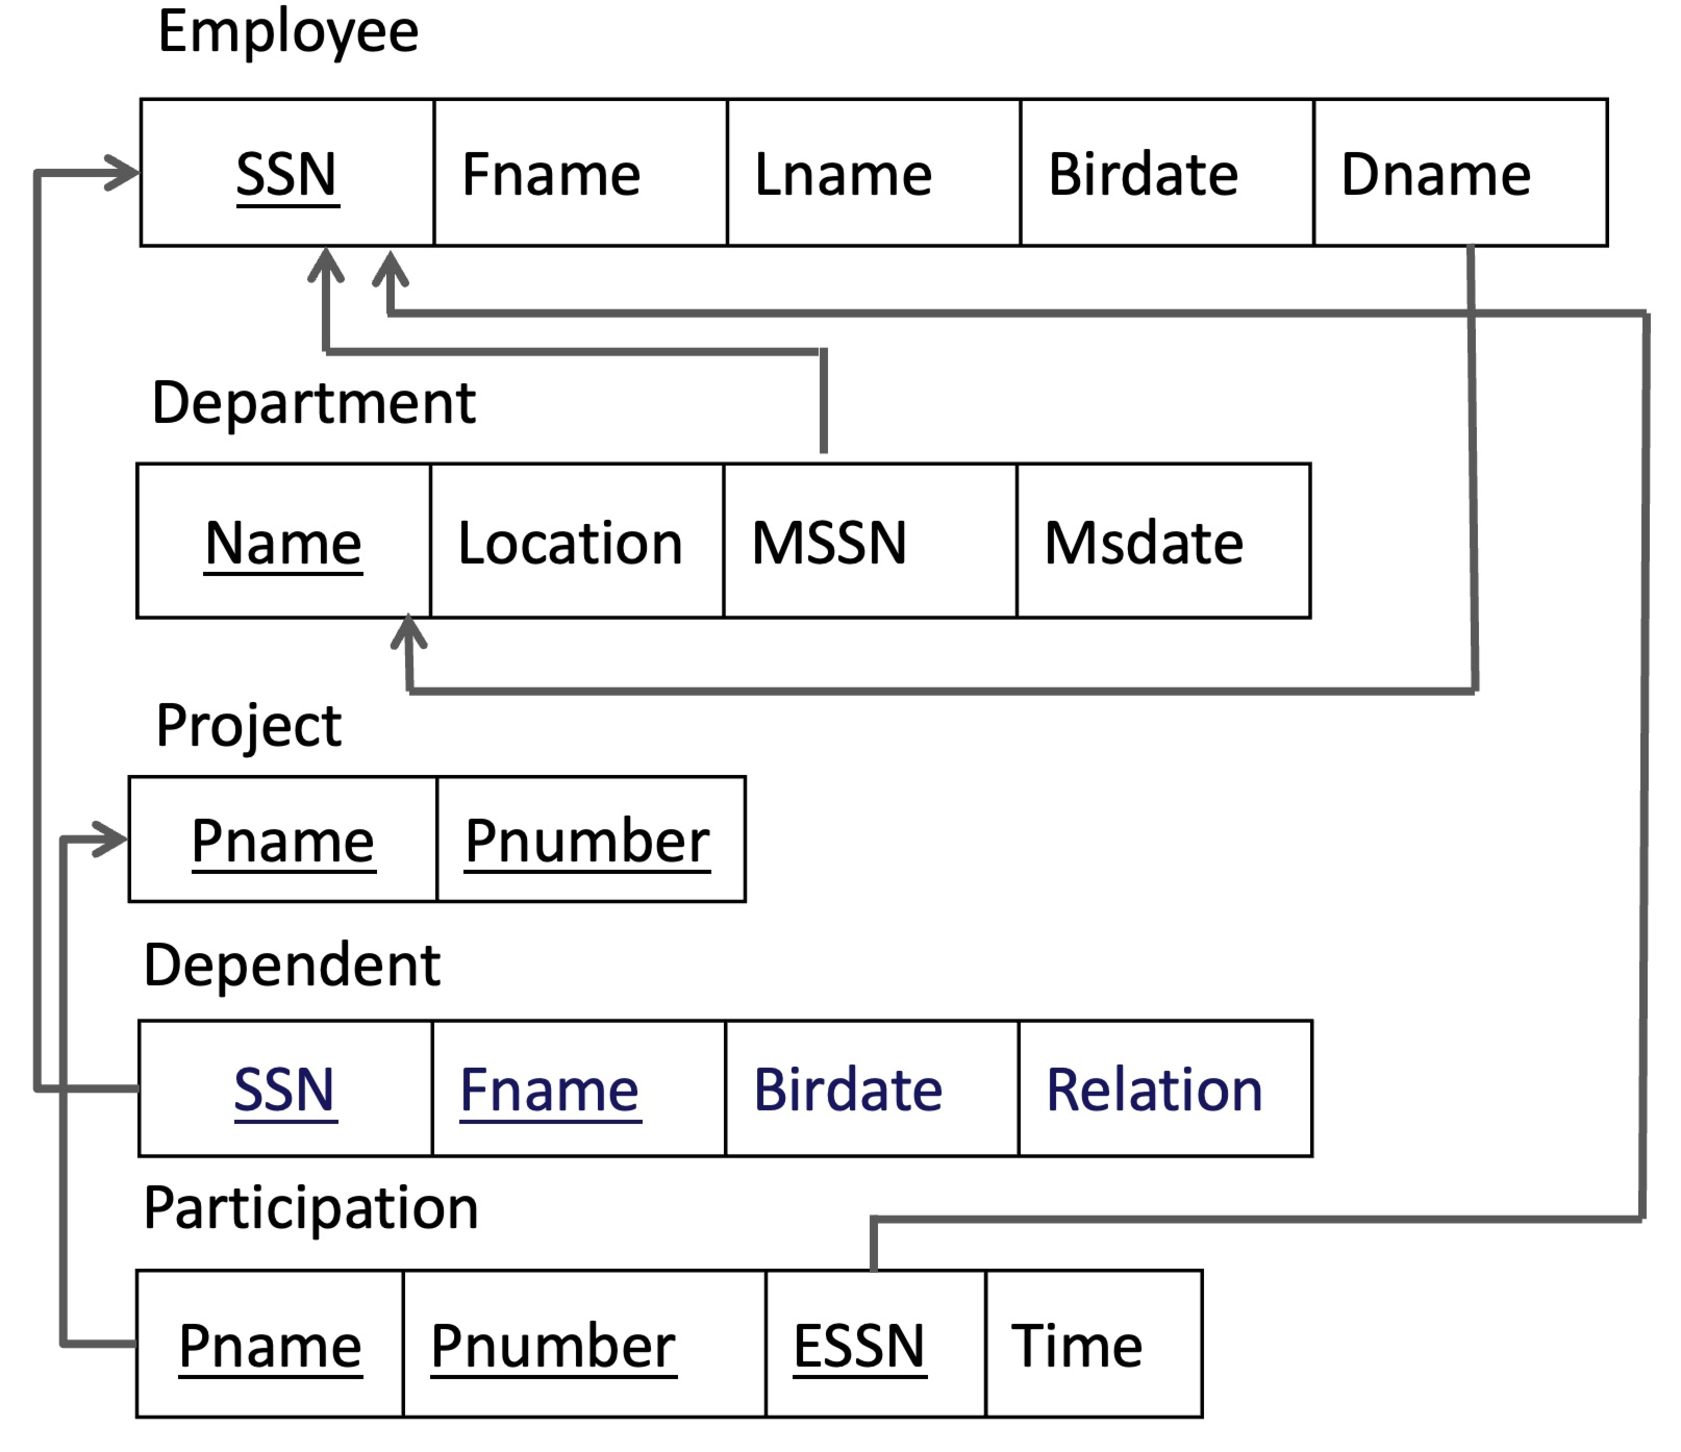
\includegraphics[width=0.4\textwidth]{Figure/Mapping2.pdf}
  \caption{Relation Schema}
\end{figure}

\section{Relational Integrity Constraints}

First, we define the \texttt{NULL} value.  

\texttt{NULL} represents an attribute whose value is unknown or does not exist for a particular entity instance. In general, it is a special marker indicating the absence of a value.  

A \textbf{foreign key} is an attribute (or a set of attributes) that stores the value of the primary key of another relation.  

Formally, a set of attributes \(FK\) in a relation schema \(R_1\) may be a foreign key if:
\begin{itemize}
  \item The attributes of \(FK\) have the same domains as the attributes of the primary key in another relation schema \(R_2\), and
  \item For every tuple \(t_1 \in R_1\), the value of \(FK\) either matches the value of the primary key in some tuple \(t_2 \in R_2\), or is \texttt{NULL}.
\end{itemize}

For each new tuple (record), the insertion is valid if:
\begin{enumerate}
  \item The primary key value does not already exist in the relation.  
  \item Each foreign key value is either entirely \texttt{NULL} or entirely non-\texttt{NULL} and occurs in the referenced relation.  
\end{enumerate}

Now, assuming our dataset is originally in a valid state, how can it become invalid? Through \textbf{insertion}, \textbf{deletion}, or \textbf{update} operations.  

There are three important \textbf{integrity constraints} in the relational model:

\begin{enumerate}
  \item \textbf{Key constraint:} Candidate key values must be unique in every relation instance.  
  \item \textbf{Entity integrity:} An attribute that is part of a primary key cannot be \texttt{NULL}.  
  \item \textbf{Referential integrity:} Ensures that foreign key values in one relation correspond to existing primary key values in another relation.  
\end{enumerate}

If any of these integrity constraints are violated, the dataset enters an invalid state.  

For example:
\begin{itemize}
  \item Inserting a tuple with a duplicate primary key or without a primary key value violates the \textbf{key} or \textbf{entity integrity} constraints.  
  \item Deleting a record that is referenced as a foreign key in another relation violates the \textbf{referential integrity} constraint.  
  \item Updating a tuple’s key value to one that causes duplication or breaks foreign key references can also result in an invalid state.  
\end{itemize}
